\subsection{Experiment Setup} \label{Experiment_Setup}

%\colorbox{orange}{\parbox{\textwidth}{I know this is more like the SUNBYTE structure and not so much like the EXIST one, but in this particular case I prefer the readability of SUNBYTE}}



%very general experiment setup
The experiments mounts a telescope with an attached CMOS sensor inside the gondola, looking out as shown in figure \ref{fig::4-1_CAD}. The telescope is mounted on a gimbal system that provides stabilisation along two axis (three if required, depending on simulation results, hardware is available) and tracking in three dimensions. The sensor/telescope/gimbal system will be shielded from the Sun's radiation and climatized in order to provide the required operation temperatures. This is achieved by using Peltier elements where heating or cooling may be necessary (e.\,g.~the sensor) and heating pads where there is only a chance of freezing (e.\,g.~the moving parts of the gimbal). The general setup with data flows can be seen in figure \ref{fig::4-1_block_diagram}. The individual sections of the experiment are described below.

\begin{figure}[h]
	\centering
	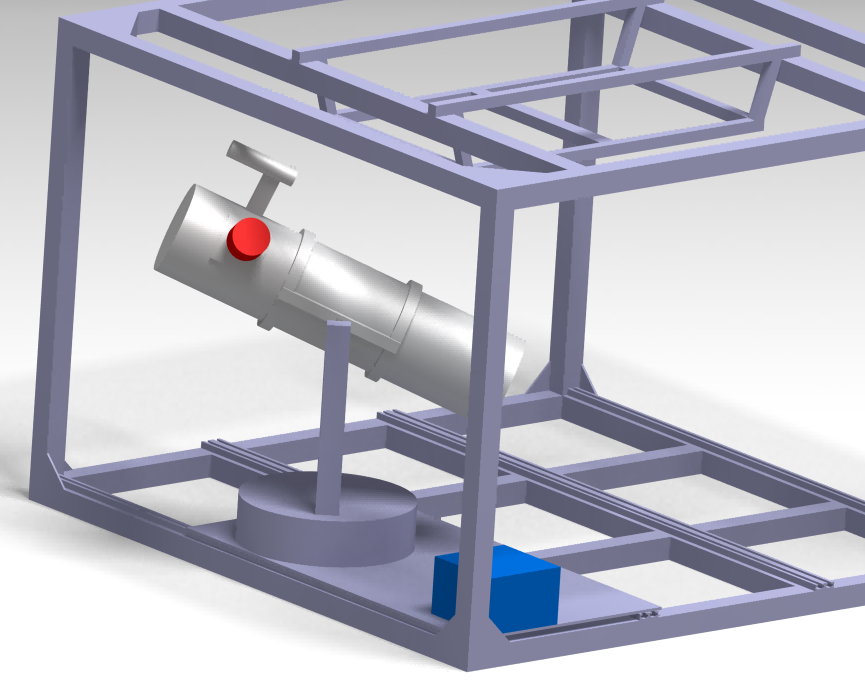
\includegraphics[width=0.7\linewidth]{4-experiment-design/img/setup/Assembly_3}
	\caption{CAD-model of the experiment}
	\label{fig::4-1_CAD}
\end{figure}


\subsubsection{Telescope and CMOS sensor}
% telescope and CMOS sensor
The telescope chosen is a Sky-Watcher~BKP~130~DS (see figure \ref{fig::4.1-telescope}), a parabolic newtonian reflector with a focal length of 650\,mm, an optical diameter of 130\,mm and therefore featuring an aperture ratio of $f/5$. 

The imaging sensor used is ZWO ASI183MM (mono) (see figure \ref{fig::4.1-sensor}), a CMOS sensor with only one channel (mono, not color) with a resolution of 20.18\,MP (5496x3672), a sensor size of 13.2x8.8\,mm (diagonal: 15.86\,mm) and a pixel size of 2.4x2.4\,$\mu$m. To limit the wavelength bandwidth imaged, an IR filter that filters out any wavelengths below 720\,nm is used in order to use the sensor as a NIR camera.

\begin{figure}[h]
	\centering
	\begin{minipage}[t]{0.4\linewidth}
		\centering
		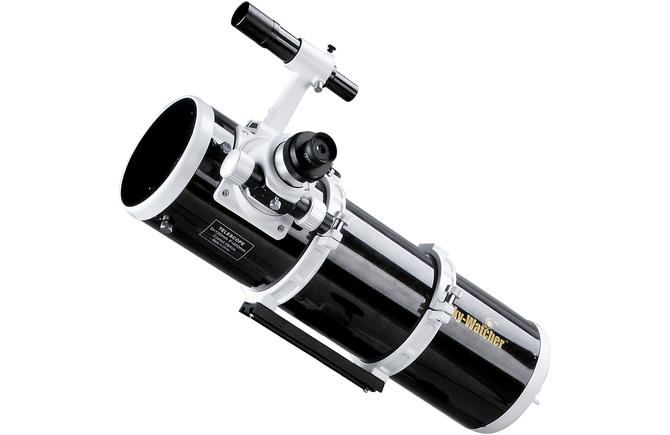
\includegraphics[width=0.8\linewidth]{4-experiment-design/img/setup/SkyWatcher_BKP130DS}
		\caption{Sky-Watcher BKP~130~DS \cite{telescope} }
		\label{fig::4.1-telescope}
	\end{minipage}
	%\hfill
	\hspace{0.1\linewidth}
	\begin{minipage}[t]{0.4\linewidth}
		\centering
		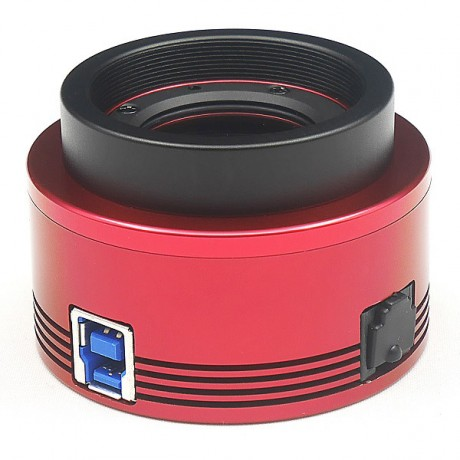
\includegraphics[width=0.5\linewidth]{4-experiment-design/img/setup/ZWO_ASI183MM}
		\caption{ZWO ASI183MM (mono) \cite{CMOS_sensor} }
		\label{fig::4.1-sensor}
	\end{minipage}
	
\end{figure}

This combination of telescope and sensor features the following specifications:

\begin{itemize}
	\item \textbf{Field of View (FoV):} the field of view determines the astronomical targets that can be observed. It depends on the sensor size and the focal length of the telescope. Naturally, there is a horizontal, a vertical and a diagonal field of view:
	\begin{align}
		\text{FoV}_\text{horizontal} &= \arctan \frac{\SI{13.2}{mm}}{\SI{650}{mm}} = \ang{1,16} \\
		\text{FoV}_\text{vertical} &= \arctan \frac{\SI{8.8}{mm}}{\SI{650}{mm}} = \ang{0,757} \\
		\text{FoV}_\text{diagonal} &= \arctan \frac{\SI{15,86}{mm}}{\SI{650}{mm}} = \ang{1,382}
	\end{align}
	\item \textbf{Sensor resolution:} the angular resolution per pixel defines the precision of the scientific data collected.
	\begin{align}
		\text{Resolution} = \arctan \frac{\SI{2,4}{\um}}{\SI{650}{mm}} %= \SI{2,1155e-4}{\degree}
		 = \ang{;;0,7616}
	\end{align}
\end{itemize}

In order to examine the field of view in case the images sent down via downlink do not show the expected astronomical targets, an additional imaging sensor is installed on a guiding telescope that has a shorter focal length than the main telescope, implying a larger field of view. With the help of these pictures it will be able to correct offset errors in the pointing mechanism of the control system due to e.\,g.~temperature drift of the sensors. In addition to this a small sanity camera with a wide angle lens (very large field of view) to keep track of the system status and detect possible errors if neither the NIR images nor the images from the guiding telescope show the expected results may be installed (not included in figures \ref{fig::4-1_CAD} and \ref{fig::4-1_block_diagram}).



\subsubsection{Electronics}

\begin{figure}[htb]
	\centering
	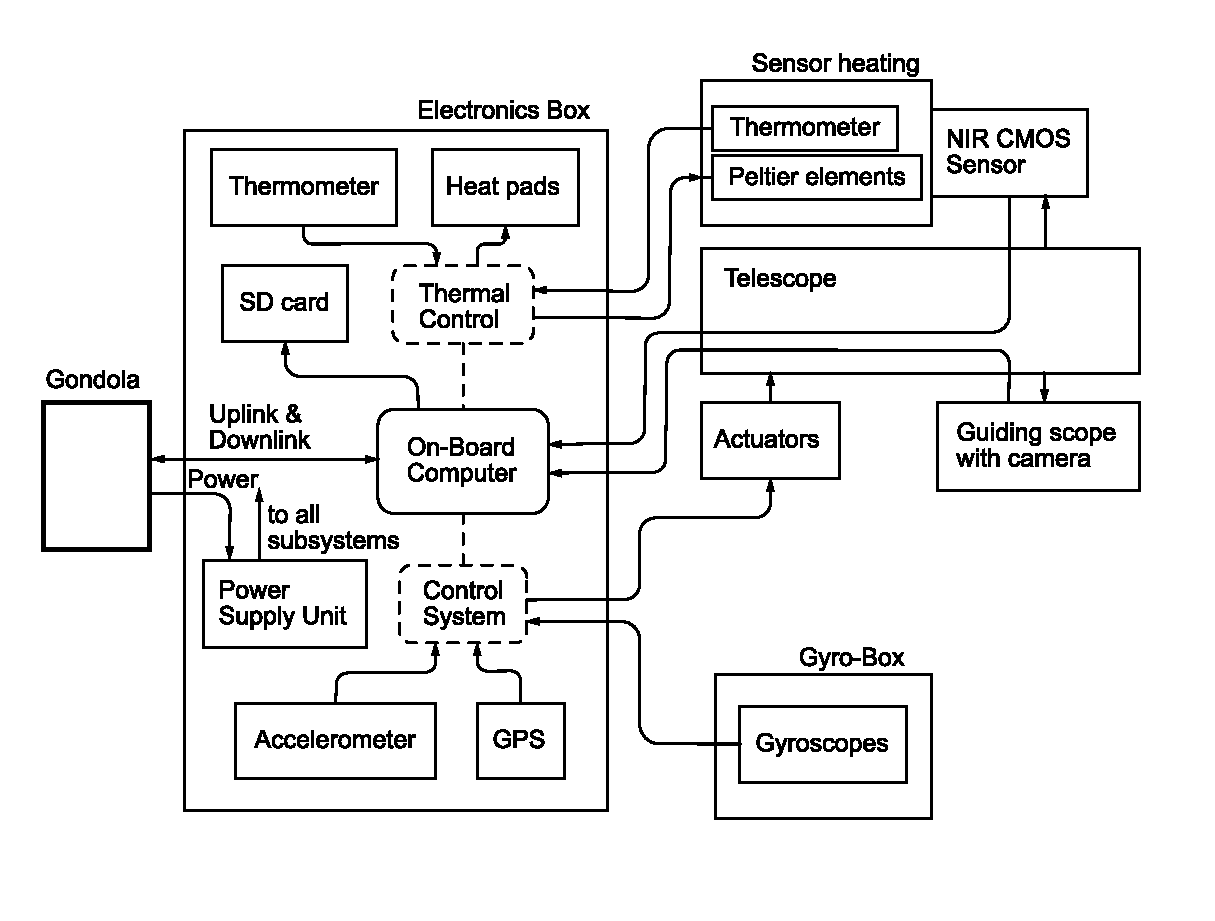
\includegraphics[width = \linewidth]{4-experiment-design/img/setup/Block_diagram_4-1}
	\caption{Block diagram of the experiment setup}
	\label{fig::4-1_block_diagram}
\end{figure}

% content of electronics box
The On-Board Computer is hosted by the electronics box that also features the onboard storage as well as the power supply unit, one set of gyroscopes and accelerometers to measure the movement of the gondola in order to provide input data to the control system, a GPS (for the control system), temperature sensors for housekeeping data and the heat management system inside the electronics box and heating elements. The sensors are located on a PCB designed by the electronics team, along with the power supply unit. In order to minimise disturbances by the power electronics and actuators, the gyroscopes are housed by a separate gyro-box that is shielded by a metal housing.



% data storage, electronics box
The CMOS sensor data is transmitted to the On-Board Computer where it is compressed with lossless compression and sent down via E-link and is also stored onboard the BEXUS balloon. The onboard storage is located in the electronics box that is designed considering compatibility with the harsh environmental conditions as well as redundancy. The mechanical structure that features the onboard storage ensures survival in case of shock due to hard impact when landing or if the BEXUS balloon lands in a lake or wetlands.

% thermal shielding - required?

\subsubsection{Control system}
% control system and actuation
The control system is responsible for tracking the target in the sky and stabilising the telescope during exposure. The tracking uses the current orientation of the gondola along the z-axis measured by a magnetometer as well as the orientation of the telescope within the gondola using encoders. Based on the current time and position (measured by the GPS system) as well as the operational field of view, the control system will select and track the target in order to point the telescope towards the astronomical targets and avoid star trails due to the sky's rotation as seen from an observer on Earth. The stabilisation system is responsible for keeping the telescope steady during exposure by counteracting the gondola movements measured by the gyrometers and accelerometers located on the sensor PCB in the electronics box.







%\colorbox{red}{currently not included: guiding scope \& camera -> needs to be included!}













































\raggedbottom